%===================================== CHAP 2 =================================

\chapter{MiBots}
An alternative to the Lithographic techniques described, is direct probing of the sample using micro manipulators. Remina Techinology Mibots are vacuum compatible micro manipulators with interchangeable tungsten probes capable of electrical probing. The \begin{wrapfigure}{r}{.5\textwidth}
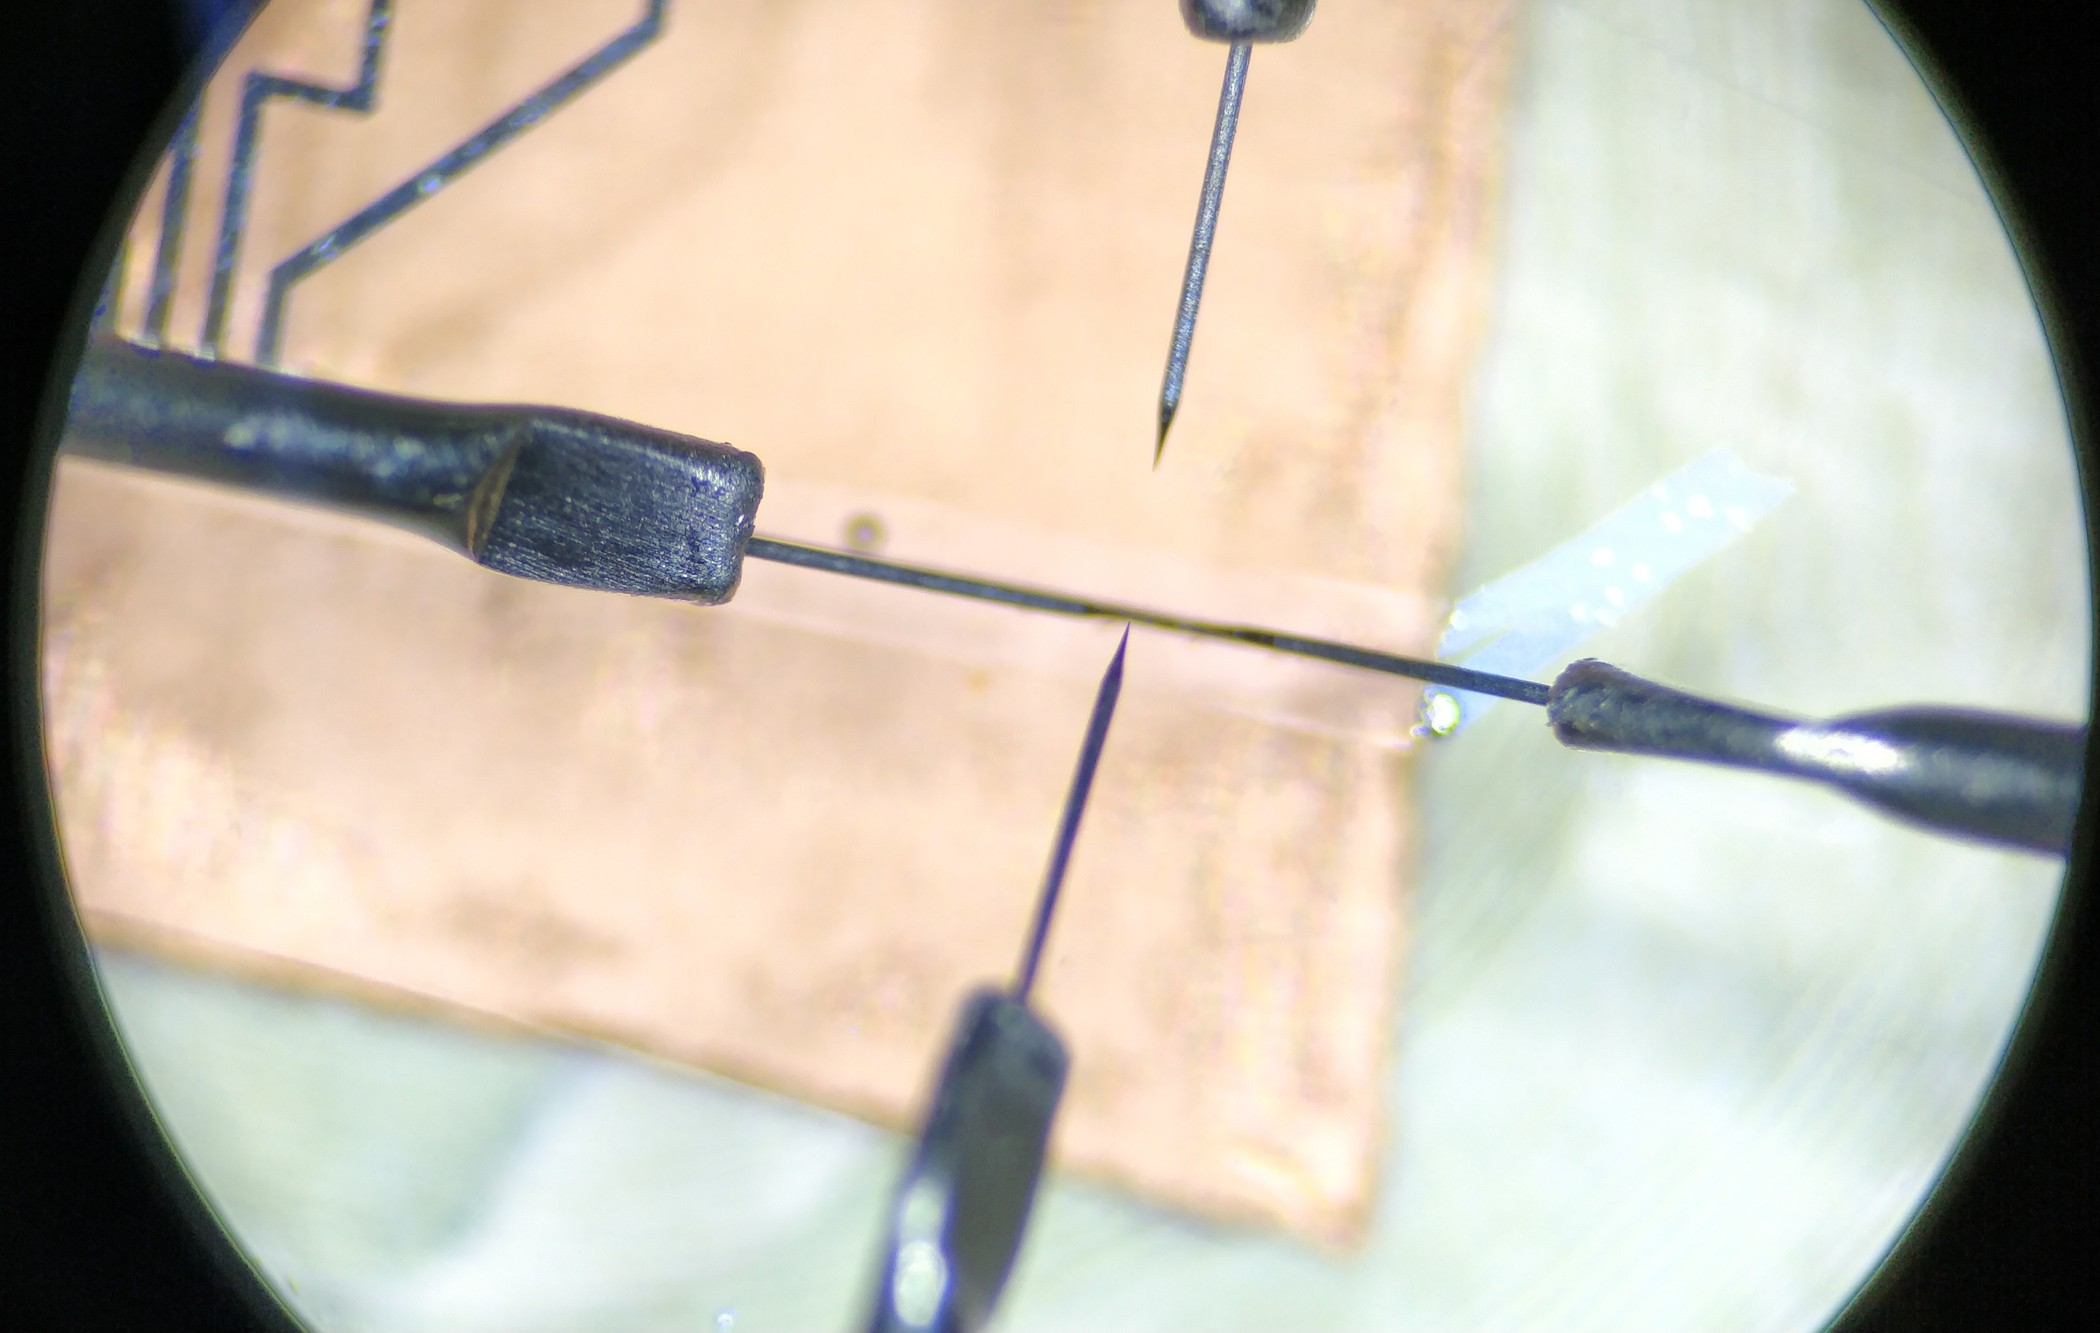
\includegraphics[width=.5\textwidth]{fig/MiBots/IMG_20190409_143016.png}
\caption{Mibot with 1 um Probe tips directly contacting the exposed sample core. The two outer current carrying probes are in contact while the voltage probes are raised above the sample.}
\end{wrapfigure} positioning precision is in the nm range making them capable of probing the smallest cores. The MiBots have a stage that can be used with an optical or electron microscope. Use with an electron microscope allows for high accuracy in the measurement of the probe spacing. Direct probing has the advantage of eliminating the challenges associated with lithography, including the need to bridge an cracking in the glass fiber and any relief profile and possible chipping at the glass epoxy interface. Problems with metal adhesion to the three different materials (glass,epoxy,core) are substrate is also eliminated. While work has been done to use micromanipulators to characterize semiconductor fibers \cite{Engel2016DirectPhotosynthesis} 
past experience in our group has found that reliable electrical contact is difficult to achieve. Ohmic contacts of the manipulators requires sufficient force (look up here). By defining contacts only on the core of the fiber, we hope to negate the problems encountered in the past. 


\cleardoublepage
